\documentclass[10pt,a4paper]{article}
\usepackage[margin=1.45cm]{geometry}
\usepackage{fontspec}
\usepackage{microtype}
\usepackage[table]{xcolor}
\usepackage{tikz}
\usetikzlibrary{positioning}
\usepackage[most]{tcolorbox}
\usepackage{enumitem}
\usepackage{tabularx}
\usepackage{booktabs}
\usepackage{amsmath,amssymb}
\usepackage{hyperref}
\usepackage{fancyhdr}
\usepackage{titlesec}
\usepackage{array}
\usepackage{ragged2e}

\setmainfont{Lato}
\setsansfont{Lato}

\definecolor{navy}{HTML}{17324D}
\definecolor{blue}{HTML}{2878B5}
\definecolor{cyan}{HTML}{34A6B8}
\definecolor{teal}{HTML}{2C8C7A}
\definecolor{orange}{HTML}{F29F4B}
\definecolor{red}{HTML}{D95D5D}
\definecolor{purple}{HTML}{7768AE}
\definecolor{lightblue}{HTML}{EDF6FC}
\definecolor{lightteal}{HTML}{EDF8F5}
\definecolor{lightorange}{HTML}{FFF5E8}
\definecolor{lightpurple}{HTML}{F3F0FA}
\definecolor{lightgray}{HTML}{F4F6F8}
\definecolor{darkgray}{HTML}{34495E}

\hypersetup{colorlinks=true,linkcolor=blue,urlcolor=blue}
\pagestyle{fancy}
\fancyhf{}
\lhead{\textcolor{navy}{\textbf{PersonaOS}}}
\rhead{\textcolor{darkgray}{Research Idea}}
\cfoot{\textcolor{darkgray}{\thepage}}
\renewcommand{\headrulewidth}{0.3pt}
\setlength{\parindent}{0pt}
\setlength{\parskip}{4pt}
\setlist[itemize]{leftmargin=*,topsep=2pt,itemsep=1.5pt}
\setlist[enumerate]{leftmargin=*,topsep=2pt,itemsep=1.5pt}

\titleformat{\section}{\Large\bfseries\color{navy}}{}{0pt}{}
\titleformat{\subsection}{\large\bfseries\color{blue}}{}{0pt}{}

\newtcolorbox{keybox}[2][]{
  enhanced, breakable, colback=#2!7, colframe=#2,
  boxrule=0.8pt, arc=2mm, left=3mm,right=3mm,top=2.5mm,bottom=2.5mm,
  fonttitle=\bfseries, #1
}
\newtcolorbox{compactbox}[1]{
  enhanced, breakable, colback=white, colframe=#1,
  boxrule=0.65pt, arc=1.8mm, left=2.5mm,right=2.5mm,top=2mm,bottom=2mm
}

\begin{document}

\begin{tcolorbox}[enhanced, colback=navy, colframe=navy, arc=3mm, boxrule=0pt,
  left=6mm,right=6mm,top=6mm,bottom=6mm]
{\fontsize{23}{27}\selectfont\bfseries\color{white} PersonaOS}

\vspace{1mm}
{\Large\color{white} One User, Many Selves}

\vspace{2mm}
{\large\color{white!88} Uncertainty-Aware, Contextual, and User-Governed Cognitive Memory for Personalized LLM Agents}

\vspace{3mm}
{\small\color{white!80} A unified extension of dynamic user profiling, implicit persona learning, active clarification, contextual personalization, cognitive memory, and user-controlled privacy.}
\end{tcolorbox}

\begin{keybox}[title=Core Idea]{blue}
PersonaOS replaces the conventional flat textual user profile with a \textbf{multi-layer belief memory}. It models not only \emph{what} the system believes about a user, but also \emph{how certain} that belief is, \emph{where it came from}, \emph{when and where it is valid}, and \emph{whether the user permits its use}. At inference time, the system selects one of four actions: \textbf{personalize}, \textbf{ask a clarification question}, \textbf{abstain from using uncertain memory}, or \textbf{provide a generic safe response}.
\end{keybox}

\section{1. Motivation and Research Gap}

Existing personalized LLM systems typically compress interaction history into a single profile such as:

\begin{compactbox}{red}
\texttt{The user prefers concise answers. The user likes vegetarian food.}
\end{compactbox}

This representation is often too rigid. It can incorrectly turn a weak signal into a permanent fact, mix the user's preferences with those of other people, ignore context, store short-lived events as stable traits, and use sensitive information without sufficient control.

\begin{tabularx}{\textwidth}{>{\bfseries\color{navy}}p{3.1cm} X}
\toprule
Problem & Why It Matters \\
\midrule
Overconfidence & Implicit or ambiguous evidence is stored as a certain fact. \\
Flat identity & A user may prefer different behavior in research, exams, work, and casual settings. \\
Forced personalization & The model answers even when the profile is uncertain or conflicting. \\
Weak user control & Users cannot reliably scope, expire, correct, or delete individual memories. \\
Mixed memory types & Events, stable traits, safety constraints, and interaction styles are stored together. \\
\bottomrule
\end{tabularx}

\begin{keybox}[title=Research Thesis]{purple}
Personalization should be formulated as \textbf{responsible belief management under uncertainty, context, and user consent}, rather than static profile retrieval or free-form summarization.
\end{keybox}

\section{2. Proposed Framework}

\begin{center}
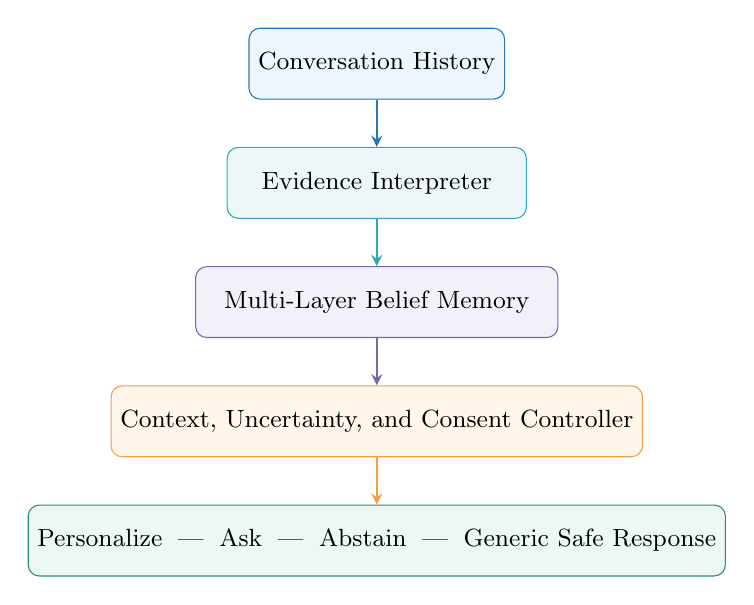
\begin{tikzpicture}[node distance=6mm, every node/.style={font=\small}, >=stealth]
\node[draw=blue, rounded corners, fill=lightblue, minimum width=3.2cm, minimum height=0.9cm] (h) {Conversation History};
\node[draw=cyan, rounded corners, fill=cyan!9, below=of h, minimum width=3.8cm, minimum height=0.9cm] (e) {Evidence Interpreter};
\node[draw=purple, rounded corners, fill=lightpurple, below=of e, minimum width=4.6cm, minimum height=0.9cm] (m) {Multi-Layer Belief Memory};
\node[draw=orange, rounded corners, fill=lightorange, below=of m, minimum width=4.8cm, minimum height=0.9cm] (c) {Context, Uncertainty, and Consent Controller};
\node[draw=teal, rounded corners, fill=lightteal, below=of c, minimum width=5.7cm, minimum height=0.9cm] (a) {Personalize \;|\; Ask \;|\; Abstain \;|\; Generic Safe Response};
\draw[->,thick,blue] (h)--(e);
\draw[->,thick,cyan] (e)--(m);
\draw[->,thick,purple] (m)--(c);
\draw[->,thick,orange] (c)--(a);
\end{tikzpicture}
\end{center}

\subsection{2.1 Evidence Interpreter}

Each new conversation chunk is converted into candidate memory claims. Every claim contains:

\begin{compactbox}{cyan}
\textbf{Claim} \;|\; \textbf{Owner} \;|\; \textbf{Evidence} \;|\; \textbf{Confidence} \;|\; \textbf{Time} \;|\; \textbf{Context} \;|\; \textbf{Sensitivity} \;|\; \textbf{Permission}
\end{compactbox}

\textbf{Example}
\begin{verbatim}
Claim: The user may prefer gluten-free meals
Owner: User
Evidence type: Implicit
Confidence: 0.61
Context: Food, travel
Temporal status: Current, unconfirmed
Sensitivity: Health-related
Permission: Use silently
\end{verbatim}

The memory updater performs one of the following operations:

\begin{center}
\fcolorbox{blue}{lightblue}{\strut ADD}\quad
\fcolorbox{teal}{lightteal}{\strut UPDATE}\quad
\fcolorbox{purple}{lightpurple}{\strut MERGE}\quad
\fcolorbox{red}{red!7}{\strut RETRACT}\quad
\fcolorbox{orange}{lightorange}{\strut EXPIRE}\quad
\fcolorbox{darkgray}{lightgray}{\strut IGNORE}
\end{center}

\subsection{2.2 Cognitive Multi-Layer Belief Memory}

\begin{tabularx}{\textwidth}{>{\bfseries\color{navy}}p{3.6cm} X}
\toprule
Memory Layer & Function \\
\midrule
Episodic Memory & Time-specific events, such as an exam next week or a recent injury. \\
Semantic Persona Memory & Stable background attributes, such as education, profession, or long-term goals. \\
Contextual Preference Memory & Preferences conditioned on role, task, audience, goal, and situation. \\
Constraint and Safety Memory & Allergies, medical restrictions, accessibility needs, and hard constraints. \\
Interaction Policy Memory & Preferred response style, explanation depth, tone, and workflow. \\
Governance and Consent Memory & Scope, retention period, mention policy, correction, and forgetting rules. \\
\bottomrule
\end{tabularx}

\begin{keybox}[title={One User, Many Selves}]{teal}
The framework does not assume one global preference per user. It learns conditional preferences such as:
\begin{itemize}
  \item \textbf{Research learning:} detailed, step-by-step explanations.
  \item \textbf{Exams:} short and direct answers.
  \item \textbf{Academic email:} formal and polished writing.
  \item \textbf{Casual chat:} natural and informal language.
\end{itemize}
These behaviors are not contradictions; they are context-dependent selves.
\end{keybox}

\subsection{2.3 Ask-or-Personalize Decision Policy}

Before generating a response, the controller checks:

\begin{itemize}
  \item Is the relevant memory sufficiently confident?
  \item Does the preference belong to the user?
  \item Is it still temporally valid?
  \item Is it valid in the current context?
  \item Is its use permitted and non-intrusive?
  \item Are multiple memories conflicting?
\end{itemize}

It then selects one action:

\begin{tabularx}{\textwidth}{>{\bfseries}p{2.8cm} X}
\rowcolor{lightblue} PERSONALIZE & Use relevant, valid, permitted, and sufficiently confident memory. \\
\rowcolor{lightorange} ASK & Ask one targeted clarification question when ambiguity materially affects the answer. \\
\rowcolor{lightpurple} ABSTAIN & Answer without using uncertain or conflicting personal information. \\
\rowcolor{lightteal} GENERIC SAFE & Provide a general response when personalization would violate privacy or consent. \\
\end{tabularx}

A lightweight utility function controls unnecessary questions:
\[
U(a)=R_{\text{personalization}}-\lambda_1C_{\text{wrong assumption}}-\lambda_2C_{\text{clarification}}-\lambda_3C_{\text{privacy}},
\quad a\in\{P,A,B,G\}.
\]

\subsection{2.4 User-Governed Memory}

Users can directly control the memory through natural language:

\begin{compactbox}{orange}
\begin{itemize}
  \item ``Remember this permanently.''
  \item ``Use this only for travel planning.''
  \item ``Do not mention this information explicitly.''
  \item ``Keep this only until next week.''
  \item ``This memory is incorrect; update it.''
  \item ``Forget this information.''
  \item ``Show me what you currently remember about me.''
\end{itemize}
\end{compactbox}

Each memory item includes a policy specifying its scope, lifetime, allowed uses, mentionability, and deletion behavior.

\section{3. Learning Strategy}

The project can be implemented without creating a new benchmark. It reuses PERSONAMEM and PERSONAMEM-V2, including existing annotations for dynamic preferences, preference ownership, implicit signals, sensitive information, and forgetting requests.

\begin{enumerate}
  \item \textbf{Memory extraction SFT:} learn structured claims from a conversation chunk.
  \item \textbf{Memory update SFT:} learn add, update, merge, retract, expire, and ignore operations.
  \item \textbf{Action selection SFT:} predict personalize, ask, abstain, or generic-safe.
  \item \textbf{Optional lightweight GRPO:} optimize the final personalized response while preserving memory correctness and policy compliance.
\end{enumerate}

A compact multi-objective reward can be used:
\[
R=R_{\text{answer}}+\alpha R_{\text{memory}}+\beta R_{\text{context}}+\gamma R_{\text{clarification}}+\delta R_{\text{consent}}-\eta R_{\text{intrusiveness}}-\mu R_{\text{size}}.
\]

\section{4. Research Questions and Hypotheses}

\begin{tabularx}{\textwidth}{>{\bfseries\color{blue}}p{1.2cm} X}
RQ1 & Does multi-layer cognitive memory outperform a single textual memory? \\
RQ2 & Does context-conditioned profiling reduce apparent preference conflicts? \\
RQ3 & Can ask-or-personalize reduce false assumptions without excessive questioning? \\
RQ4 & Can user-governed memory reduce privacy and consent violations? \\
RQ5 & Can the system distinguish temporary events, stable traits, preferences, and hard constraints? \\
\end{tabularx}

\begin{keybox}[title=Main Hypotheses]{blue}
\begin{itemize}
  \item Multi-layer memory improves personalized response accuracy and memory faithfulness.
  \item Contextual profiles reduce wrong-style and wrong-preference activation.
  \item Active clarification lowers incorrect assumptions with a small interaction cost.
  \item Policy-aware memory sharply reduces unauthorized use of sensitive information.
  \item Confidence-aware memory improves calibration and reduces hallucinated user attributes.
\end{itemize}
\end{keybox}

\section{5. Evaluation Plan}

\begin{tabularx}{\textwidth}{>{\bfseries\color{navy}}p{3.8cm} X}
\toprule
Evaluation Dimension & Metrics \\
\midrule
Personalization & MCQ accuracy, open-ended preference alignment, response quality. \\
Profile quality & Claim accuracy, ownership accuracy, dynamic update accuracy, hallucinated attribute rate. \\
Context sensitivity & Contextual preference accuracy, false conflict rate, role selection accuracy. \\
Uncertainty & Expected Calibration Error, Brier score, selective accuracy. \\
Clarification & Decision accuracy, unnecessary question rate, final accuracy after clarification. \\
User control & Forgetting compliance, scope compliance, consent violation rate, sensitive information leakage. \\
Efficiency & Memory size, compression ratio, update cost, and inference latency. \\
\bottomrule
\end{tabularx}

\subsection{Baselines and Ablations}

\begin{itemize}
  \item Full-context prompting, RAG, Mem0, and PERSONAMEM-V2 Agentic Memory.
  \item Single free-form textual memory.
  \item Multi-layer memory without uncertainty.
  \item Multi-layer memory without contextualization.
  \item Multi-layer memory without clarification.
  \item Multi-layer memory without governance.
  \item Full PersonaOS.
\end{itemize}

\section{6. Key Experiments}

\begin{enumerate}
  \item \textbf{One User, Many Selves:} evaluate whether the correct context-specific preference is activated.
  \item \textbf{Ask or Assume:} test ambiguous ownership, hypothetical statements, and weak evidence.
  \item \textbf{Memory Editing:} verify correction, retraction, expiration, and forgetting.
  \item \textbf{Scoped Consent:} restrict a memory item to specific tasks and test unauthorized use elsewhere.
  \item \textbf{Memory Layer Ablation:} measure the contribution of each cognitive layer.
\end{enumerate}

\section{7. Expected Contributions}

\begin{keybox}[title=Contribution 1: New Formulation]{purple}
Personalization as multi-layer belief management under uncertainty, context, and consent.
\end{keybox}

\begin{keybox}[title=Contribution 2: New Memory Architecture]{cyan}
A cognitive memory that separates episodes, stable traits, contextual preferences, constraints, interaction policies, and governance rules.
\end{keybox}

\begin{keybox}[title=Contribution 3: Active Decision Policy]{orange}
A practical ask-or-personalize controller that avoids confident but incorrect personalization.
\end{keybox}

\begin{keybox}[title=Contribution 4: User Control]{teal}
Editable, scoped, expiring, and forgettable memories with explicit user-defined permissions.
\end{keybox}

\section{8. Scope and Feasibility}

The core paper remains focused on three components:

\begin{center}
\fcolorbox{purple}{lightpurple}{\parbox{0.29\textwidth}{\centering\textbf{1. Multi-Layer Contextual Memory}}}\hfill
\fcolorbox{orange}{lightorange}{\parbox{0.29\textwidth}{\centering\textbf{2. Ask-or-Personalize Policy}}}\hfill
\fcolorbox{teal}{lightteal}{\parbox{0.29\textwidth}{\centering\textbf{3. User-Governed Consent}}}
\end{center}

The first implementation does not require a new large-scale dataset, a full POMDP, a Bayesian neural model, or expensive multi-stage RL. Structured prompting and SFT provide a strong minimum viable system; lightweight GRPO can be added for the final version.

\begin{tcolorbox}[enhanced, colback=navy, colframe=navy, arc=2.5mm, boxrule=0pt,
left=4mm,right=4mm,top=3.5mm,bottom=3.5mm]
\centering
{\large\bfseries\color{white} Final Vision}

\vspace{1mm}
{\color{white!90} A personalized agent should know not only who the user is, but also which version of the user is relevant now, how certain that belief is, and whether it is allowed to use it.}
\end{tcolorbox}

\end{document}
